% !TEX root = ./projekt.tex
%=========================================================================
% (c) Michal Bidlo, Bohuslav Křena, 2008

\chapter{Úvod}

\chapter{Definice a pojmy}

\section{Teorie množin}

\section{Teorie grafů}
\begin{defn}
  (Strom). \cite[str. 12]{Koutny}\\
  Strom je orientovaný acyklický graf, $G = (\Sigma, R)$, který má tyto
  tři vlastnosti: \\
  \indent
  $G$ má právě jeden uzel, do něhož nevstupují žádné hrany;
  tento uzel se nazývá kořen $G$ označovaný jako kořen($G$).\\
  \indent
  Jestliže $a \in \Sigma$ a $a \neq$ kořen($G$), potom $a$ je
  potomkem kořenu($G$) a vstupuje do něj právě jedna hrana.\\
  \indent
  Každý uzel $a \in \Sigma$ který není listem má svého přímého potomka,
  $b_1$ až $b_n$, řazené zleva doprava tak, že $b_1$ je
  nejlevějším přímým potomkem $a$ a $b_n$ je nejpravějším přímým
  potomkem $a$.
\end{defn}

\begin{defn}
  (Úroveň, cesta, řez, hranice, hloubka, elementární strom a podstrom). \cite[str. 12]{Koutny}\\
  Nechť $G = (\Sigma, R)$ je stromem.\\
  \indent
  Úroveň $l$, stromu $G$, je posloupnost $s$,
  všech uzlů se stejnou vzdáleností od kořene($G$).
  Jinými slovy, úroveň $l$, je posloupnost, $s = n_1 n_2 ... n_k$,
  taková, že existuje cesta v grafu o délce $\ell$ v $G$
  pro všechny posloupnost od kořene($G$)
  $ ... n_i$, pro $1 \leq i \leq k$ a $l \geq 1$.\\
  \indent
  Cesta $p$, stromu $G$, je posloupnost $s$, uzlů,
  kde první uzel je kořen($G$), poslední je listem a mezi každými
  dvěma následnými uzly v $s$ existuje hrana v $G$.
  Jinými slovy, cesta $p$ stromu $G$, je posloupnost,
  $s = n_1 n_2 ... n_k$, taková, že $s$ je cesta grafem
  o délce $k$ v $G$, kde $n_1 =$ kořen($G$) a $n_k$ je listem
  v $G$, pro $k \geq 1$.\\
  \indent
  Řez $c$, stromu $G$ je posloupnost $s$, uzlů takových,
  že každá cesta v $G$ má právě jeden uzel v $c$.
  Jinými slovy, řez $c$ je posloupnost, $s = n_1 n_2 ... n_k$,
  taková, že pro každou cestu $p = m_1 m_2 ... m_\ell$ stromu $G$,
  $|\{n_1, n_2, ..., n_k\} \cap \{m_1, m_2, ..., m_\ell\}| = 1$,
  pro $k, \ell \geq 1$.\\
  \indent
  Hranice stromu $G$, hranice($G$),
  je posloupnost listů $G$ řazených zleva do prava.\\
  \indent
  Hloubka stromu $G$, hloubka($G$), je délka nejdelší cesty v $G$;
  jestliže platí hloubka($G$)$ = 1$, potom je $G$ elementární strom.\\
  \indent
  Jestliže $G' = (\Sigma', R')$ představuje strom vyhovující těmto
  čtyřem podmínkám:
  $\Sigma' \neq \emptyset$;
  $\Sigma' \subseteq \Sigma$;
  $R' = (\Sigma' \times \Sigma')$;
  a jestliže v $G$ není žádný z uzlů v $\Sigma - \Sigma'$ potomkem
  uzlu v $\Sigma'$, potom je $G'$ podstromem $G$.
\end{defn}

\chapter{Formální jazyky}

Teorie formálních jazyků si bere za cíl formalizovat jazyky
(přirozené, programovací, matematické, ...) tak, abychom se mohli zabývat jejich
automatizovaným zpracováním.
Pojmy, které známe z lingvistiky jsou zde zobecněny a přesně definovány,
takže nemusí úplně odpovídat naší dosavadní představě.

\subsubsection*{Abeceda}

Základem jazyka je \term{abeceda}. V teorii formálních jazyků je obvykle značena
$\Sigma$ (sigma) a je definována jako konečná neprázdná množina, jejíž objekty
se nazývají \term{symboly}.

\subsubsection*{Řetězec}

Konečná posloupnost symbolů patřících do $\Sigma$ je \term{řetězec} nad $\Sigma$.
Zvláštním případem je $\varepsilon$ (epsilon), značící \term{prázdný řetězec} -
tedy takový, že neobsahuje žádný symbol.

\subsubsection*{Jazyk}

$\Sigma^*$ značí množinu všech řetězců, které je možné sestrojit nad abecedou $\Sigma$.
Jakákoliv podmnožina $L \subseteq \Sigma^*$ je \term{jazykem} nad abecedou $\Sigma$.
Jestliže \term{jazyk} představuje konečnou množinu řetězců, potom jej nazýváme \term{konečným jazykem},
v opačném případě \term{jazykem nekonečným}.

\subsubsection*{Gramatika}

Pokud se zabýváme nekonečnými jazyky, nemůžeme je vyjádřit jednoduchým výčtem jejich
řetězců. Místo toho definujeme \term{gramatiku}, která stanovuje pravidla pro generování
řetězců patřících do daného jazyka.\\

\noindent
\term{Gramatika} obecně obsahuje 4 části:
\begin{itemize}
  \item Množinu \term{neterminálních symbolů} $N$ (neterminálů), které slouží k označení syntaktických celků.
  \item Množinu \term{terminálních symbolů} $\Sigma$ (terminálů) - symboly, které jsou konečným výstupem. (abeceda)
  \item Množinu přepisovacích pravidel $P$.
  \item Počáteční (startovací) symbol $S \in N$.
\end{itemize}

\subsubsection*{Přepisovací pravidla}
\label{term:rewriteRule}

\term{Přepisovací pravidlo} je složeno ze dvou řetězců $(\alpha, \beta)$,
složených z terminálů a neterminálů, přičemž $\alpha$ obsahuje alespoň jeden neterminál.
Zapisují se jako $\alpha \rightarrow \beta$.\\
Pravidla se aplikují od startovacího symbolu, kdy postupně přepisujeme řetězec tak že nahradíme
jakoukoliv část řetězce, která se nachází na levé straně některého pravidla za pravou stranu tohoto pravidla.
Tato operace se také nazývá \term{derivace}.
Řetězec upravujeme podle pravidel tak dlouho, až se v něm nacházejí pouze neterminály.

\begin{figure}[H]
  \centering
  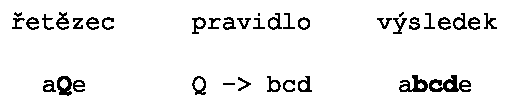
\includegraphics{fig/rewriteRule.pdf}
  \caption{Příklad derivace podle pravidla}
  \label{img:rewriteRule}
\end{figure}

\subsubsection*{Ekvivalence gramatik}
Dvě gramatiky označujeme jako \term{ekvivalentní}, pokud generují stejný jazyk.

\subsubsection*{Výpočetní model}

Výpočetní model lze definovat jako hypotetický přístroj,
který využíváme k řešení daného problému. Vlastnosti modelu určují,
jak sofistikované problémy je schopen řešit.

\subsubsection*{Hierarchie jazyků} \label{chomsky:hierarchy}

Omezením gramatiky lze zaručit to, že ji lze zpracovávat jednodušším
\term{Výpočetním modelem}. Jazyky se proto
dělí do tříd právě podle toho, jaký výpočetní model je dokáže zpracovat.\\

\noindent
Jedno z nejznámějších rozdělení je podle tzv. \term{Chomského hierarchie}:

\begin{itemize}
  \item \textbf{Gramatiky typu 0} (frázové/neomezené gramatiky)\\
  Zahrnují všechny formální gramatiky.\\
  Model pro zpracování se nazývá \term{Turingův stroj}.\\
  Tvoří třídu \term{rekurzivně spočetných jazyků}, zkratka \textbf{RE}.

  \item \textbf{Gramatiky typu 1} (kontextové gramatiky)\\
  Tyto gramatiky se skládají z pravidel typu $\alpha A\beta \rightarrow \alpha \gamma \beta$,
  kde $A$ je neterminál a $\alpha, \beta, \gamma$ jsou řetězce terminálů i neterminálů,
  přičemž $\gamma$ je neprázdný.\\
  Model pro zpracování se nazývá \term{lineárně ohraničený Turingův stroj}.\\
  Tvoří třídu \term{kontextových jazyků}, zkratka \textbf{CS}.

  \item \textbf{Gramatiky typu 2} (bezkontextové gramatiky)\\
  Skládají se z pravidel typu $A \rightarrow \gamma$, kde $A$ je neterminál a
  $\gamma$ řetězec terminálů a neterminálů.\\
  Model pro zpracování se nazývá \term{nedeterministický zásobníkový automat}.\\
  Tvoří třídu \term{bezkontextových jazyků}, zkratka \textbf{CF}.

  \item \textbf{Gramatiky typu 3} (regulární gramatiky)\\
  Skládají se z pravidel typu $A \rightarrow B$ a $A \rightarrow aB$,
  kde $A, B$ jsou neterminály a $a$ je terminál.\\
  Model pro zpracování se nazývá \term{konečný automat}.\\
  Tvoří třídu \term{regulárních jazyků}, zkratka \textbf{REG}.
\end{itemize}

\subsubsection*{Vyjadřovací síla jazyka}

Čím větší má jazyk vyjadřovací sílu, tím detailnější omezení je jeho
gramatika schopna klást na přijímané řetězce. Jsme tedy schopni jemněji rozlišovat,
které řetězce patří do jazyka a které ne.

V \term{Chomského hierarchii} jsou jazyky uspořádány tak, že slabší jazyk je
vždy podmnožinou silnějšího. Tedy například mezi Bezkontextové jazyky patří i
všechny Regulární jazyky.\\

\begin{figure}[H]
  \centering
  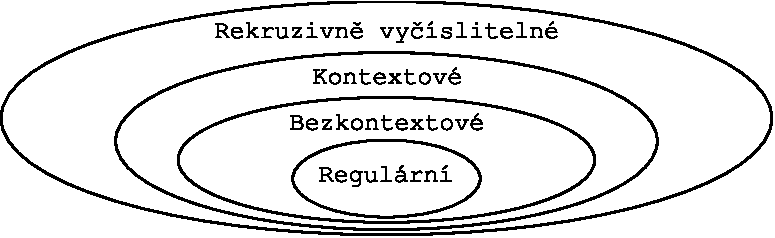
\includegraphics{fig/Chomsky.pdf}
  \caption{Schématické znázornění Chomského hieararchie}
\end{figure}


V této práci se budeme zabývat skupinami 2 a 3,
tedy bezkontextovými a regulárními jazyky. Tyto jazyky jsou prodrobněji
popsány v následujících kapitolách.

\section{Regulární jazyky}

Regulární jazyky jsou nejjednodušší formální jazyky v Chomského hierarchii.
I přesto si však našly široké využití v různých oblastech informačních technologií.
Využívají se např. pro pokročilé vyhledávání v textu nebo
pro rozdělení programovacího jazyka na základní jednotky.
V implementační části této práce jsou využity ke kontrole úrovní derivačního stromu,
také proto se jimi budeme hlouběji zabývat.

\begin{defn}
  (Regulární jazyk)\\
  Regulární jazyk nad abecedou $\Sigma$ lze definovat následovně:
  \begin{itemize}
    \item Prázdný jazyk $\emptyset$ je regulární.
    \item Pro každé $a$ z $\Sigma$ je $\{ a \}$ regulární.
    \item Jestliže $A$ a $B$ jsou regulární jazyky, poté všechny tyto jazyky jsou také regulární:
    $A \cup B$ (sjednocení), $AB$ (konkatenace) a $A^*$ (iterace).
  \end{itemize}
\end{defn}

\subsection{Konečné automaty}
Každý Regulární jazyk lze zpracovávat konečným automatem a každý konečný automat
lze vyjádřit regulárním jazykem.\\

Automat je pětice $M = (Q, \Sigma, R, s, F)$, kde:
\begin{itemize}
  \item $Q$ je množina stavů
  \item $\Sigma$ je \term{vstupní abeceda}
  \item $R$ je množina \term{přechodových pravidel}
  \item $s$ je \term{počáteční stav}
  \item $F$ je množina \term{konečných stavů}
\end{itemize}

Přechodová pravidla jsou ve tvaru $qa \rightarrow p$, kde $q, p$ jsou stavy a
$a$ je vstupní symbol. Pravidlo nám říká, že jsme-li ve stavu $q$ a na vstupu
máme symbol $a$, poté může automat přejít do stavu $p$.
Začínáme vždy v počátečním stavu a aby vstupní řetězec patřil do jazyka,
musíme skončit v jednom z konečných stavů.
Velkou výhodou je, že práce konečného automatu je paměťově velmi nenáročná, jelikož obsahuje pouze informaci o aktuálním
stavu.

\begin{exmp}
  Mějme konečný automat M1:
  \begin{lstlisting}
  M1 = (
    {s, q, f},        (* // množina stavů *)
    {a, b, c},        (* // abeceda *)
    {                 (* // množina pravidel *)
      sa $\rightarrow$ q1,
      qb $\rightarrow$ q,
      qc $\rightarrow$ f
    },
    s,                (* // počateční stav *)
    {f}               (* // množina ukončujících stavů *)
  )
  \end{lstlisting}
  A řetězec:
\begin{lstlisting}
  abbc
\end{lstlisting}

\noindent
Při kontrole vstupního řetězce budeme postupovat následovně:

\begin{enumerate}
  \item Nastavíme počáteční stav $s$
  \item Vstupním symbolem je 'a' - podle prvního pravidla přejdeme do stavu $q$
  \item Vstupním symbolem je 'b' - zůstáváme ve stavu $q$ (pr. 2)
  \item Vstupním symbolem je 'b' - zůstáváme ve stavu $q$ (pr. 2)
  \item Vstupním symbolem je 'c' - přejdeme do stavu $f$ (pr. 3)
  \item Jsme na konci řetězce - zkontrolujeme, zdali jsme v konečném stavu - řetězec byl automatem přijat,
  takže řetězec patří do jazyka generovaného automatem.
\end{enumerate}

\noindent
Během činnosti konečného automatu mohou nastat tyto chyby:

\begin{itemize}
  \item vstupní symbol nepatří do abecedy
  \item neexistuje pravidlo pro vstupní symbol a aktuální stav
  \item po přečtení posledního znaku se nenacházíme v konečném stavu
\end{itemize}
Ve všech těchto případech není vstupní řetězec přijat konečným automatem, tudíž nepatří
do jazyka generovaného automatem.\\

\noindent
Tento konečný automat lze také zobrazit pomocí následujícího grafu:

\begin{figure}[H]
  \centering
  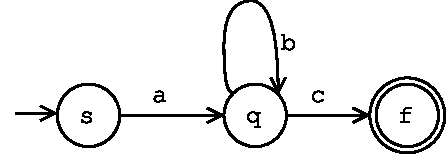
\includegraphics{fig/finiteAutomat.pdf}
\end{figure}

\end{exmp}

\noindent
Uveďme další příklad, který už nebude tak jednoduchý:
\begin{exmp}
  Mějme konečný automat M2:
  \begin{lstlisting}
  M2 = (
    {s, q1, q2, p1, p2, f1, f2},
    {a, b, c, d},
    {
      sa $\rightarrow$ q1,
      q1b $\rightarrow$ q2,
      q2c $\rightarrow$ f1,
      q1$\varepsilon$ $\rightarrow$ p1,
      p1b $\rightarrow$ p2,
      p2d $\rightarrow$ f2
    },
    s1,
    {f1}
  )
  \end{lstlisting}

  Za pozornost stojí hlavně čtvrté pravidlo s $\varepsilon$ přechodem.
  Toto pravidlo značí, že lze bez přijetí jakéhokoliv znaku přejít z jednoho stavu
  do druhého. Tyto pravidla se bohužel mohou v obecných gramatikách vyskytovat a
  způsobují potíže při zpracovávání automatu, jak bude vysvětleno dále.\\

  \noindent
  Pro větší názornost budeme nyní pracovat se schématem automatu:

  \begin{figure}[H]
    \centering
    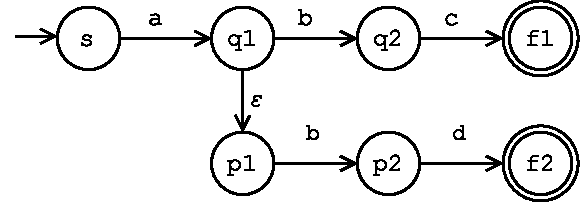
\includegraphics{fig/finiteAutomat1.pdf}
  \end{figure}

  Pokud se při zpracování ocitneme ve stavu $q1$ a vstupním symbolem bude 'b',
  není jasné, jestli máme použít 2. nebo 4. pravidlo. Museli bychom vyzkoušet jít oběma cestami
  a až zpětně bychom zjistili, která možnost byla správná. Tomuto jevu se v teorii
  formálních jazyků říká \term{nedeterminismus} a setkáme
  se s ním ještě několikrát.\\

  Nutno ale podotknout, že \term{nedeterminismus} neznamená to, že bychom nebyli schopni
  určit, jestli řetězec patří do daného jazyka. Ve skutečnosti totiž můžeme
  vyzkoušet všechna možná pravidla a zjistit, jestli z nich některé povede k úspěchu.
  Tato technika se také pro některé jazyky využívá a při zpracování
  přirozených jazyků se jí většinou nelze úplně vyhnout.
  Slepé zkoušení pravidel však vede k velkému zpomalení vyhodnocování,
  může totiž dojít k tomu, že se program bude větvit opakovaně
  a zpracování může dojít až k exponencionální složitosti.
  Např. programovací jazyky bývají navrženy tak, aby šly zpracovávat deterministicky,
  protože rychlost překladu je velmi důležitým faktorem pro jejich nasazení.

\end{exmp}

\subsection{Determinizace konečného automatu}

Z výše uvedených odstavců je zjevné, že je lepší se preventivně nedeterminismu
zbavit. Nejprve ukážeme demonstraci na tomto konkrétním příkladě a poté uvedeme
obecný algoritmus.\\

Abychom se zbavili $\varepsilon$ přechodů musíme vytvořit nový automat, který ale
generuje stejný jazyk (přijímá stejné řetězce)
jako ten původní. Takovéto dva automaty se označují jako \term{ekvivalentní}.
Protože můžeme z přechodu $q1$ kdykoliv přejít do $q2$ intuitivním řešením
je oba stavy spojit do jednoho. Pro zachování \term{ekvivalence}, musíme
do nového stavu přidat všechna pravidla, která vycházela z původních dvou stavů.
Nový automat bude vypadat takto:

\begin{figure}[H]
  \centering
  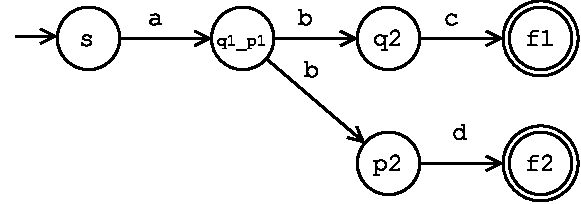
\includegraphics{fig/finiteAutomat1_1.pdf}
\end{figure}

Pokud si nové schéma dobře prohlédneme, odhalíme další zádrhel, který se nám
objevil v novém pravidle $q1\_p1$. Pokud je v tomto stavu na vstupu symbol 'b',
nevíme které pravidlo použít a máme tu opět \term{nedeterminismus}.
I tento problém lze naštěstí vyřešit obdobným způsobem:

\begin{figure}[H]
  \centering
  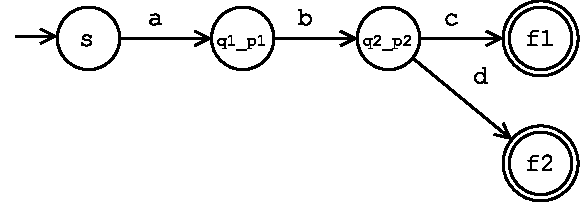
\includegraphics{fig/finiteAutomat1_2.pdf}
\end{figure}

\noindent
Tento automat můžeme označit jako \term{deterministický} a lze jej
s klidem implementovat.

\noindent
V tomto konkrétním případě jsme si pomohli intuicí, uveďme ale obecné algoritmy:\\

\begin{algorithm}[H]
  \caption{Stavy dostupné bez čtení ze stavů $E$ (\term{$\varepsilon$-uzávěr(E)})}
  \KwIn{Končný automat $M = (Q, \Sigma, R, s, F)$ a $E \subseteq Q$}
  \KwOut{\term{$\varepsilon$-uzávěr(E)}}

  \BlankLine
  \Begin{
    $\varepsilon$-uzávěr$(E)$ := $E$\;
    \Repeat{$\varepsilon$-uzávěr$(E)$ nebyl změněn}{
      $\varepsilon$-uzávěr$(E)$ := $\varepsilon$-uzávěr$(E)$ $\cup$ $\{p| q \rightarrow p
        \in R$ \And $q \in \varepsilon$-uzávěr$(E)\}$
    }
  }
\end{algorithm}

\vspace{0.5cm}

\begin{algorithm}[H]
  \caption{Odstranění $\varepsilon$ pravidel}
  \KwIn{Končný automat $I = (Q_I, \Sigma_I, R_I, s_I, F_I)$ a $E \subseteq Q$}
  \KwOut{Konečný automat bez $\varepsilon$ pravidel $O$, ekvivalentní s $I$}

  \BlankLine
  \Begin{
    $Q_O$ := $Q_I$\;
    $\Sigma_O$ := $\Sigma_I$\;
    $s_O$ := $s_I$\;
    $F_O := \{q| q \in Q_I, \varepsilon$-uzávěr$(q) \cap F_I \neq \emptyset\}$\;
    $R_O := \{qa \rightarrow p | q \in Q_I, \And \in \Sigma_I, oa \rightarrow p
      \in R_I$ pro všechna $o \in \varepsilon$-uzávěr$(q)$ v $I\}$
  }
\end{algorithm}

\vspace{0.5cm}

\begin{algorithm}[H]
  \caption{Odstranění nedeterminismu}
  \KwIn{Končný automat bez $\varepsilon$-přechodů $M = (Q, \Sigma, R, s, F)$}
  \KwOut{Deterministický KA: $D = (Q_D, \Sigma, R_D, s_D, F_D)$ ekvivalentní s $M$}

  \BlankLine
  \Begin{
    $s_D := \{s\}$\;
    $Q_{new} := \{s_D\}$\;
    $R_D := \emptyset$\;
    $Q_D := \emptyset$\;
    $F_D := \emptyset$\;
    \Repeat{$Q_{new} = \emptyset$} {
      nechť $Q' \in Q_{new}$\;
      $Q_{new} := Q_{new} - \{Q'\}$\;
      $Q_D := Q_D \cup {Q'}$\;
      \ForAll{$a \in \Sigma$}{
        $Q'' := \{q | p \in Q', pa \rightarrow q \in R\}$\;
        \If{$Q'' \neq \emptyset$}{
          $R_D := R_D \cup \{ Q' a \rightarrow Q'' \}$\;
        }
        \If{$Q'' \notin Q_D \cup \{\emptyset\}$}{
          $Q_{new} := Q_{new} \cup \{Q''\}$\;
        }
      }
      \If{$Q' \cap F \neq \emptyset$}{
        $F_D := F_D \cup \{ Q'\}$
      }
    }
  }
\end{algorithm}

\vspace{0.5cm}

Tyto algoritmy jsou definovány pro jakýkoliv Konečný automat, tedy jakýkoliv KA
lze převést na Deterministický KA \cite[str. 39]{MedunaIFJ}.
Z toho vyplývá, že jakýkoliv Regulární jazyk lze zpracovávat deterministicky,
což u jazyků z ostatních tříd \term{Chomského hierarchie} neplatí.\\

Existují také další transformace Konečného automatu, jako např.
odstranění nedostupných stavů nebo minimalizace. V této práci však
nebudou využívány a proto zde nejsou více rozebírány.\\

\subsection*{Na co konečné automaty nestačí}

\begin{exmp}
  \label{exmp:brackets}

  Řekněme, že chceme konečným automatem kontrolovat,
  jestli matematický výraz obsahuje stejné množství
  otevíracích závorek jako uzavíracích a jestli jsou ve správném pořadí.\\
  Příklady řetězců:
  \begin{itemize}
    \item '(())' - v pořádku
    \item '(()())' - v pořádku
    \item '(()' - špatně
    \item ')(' - špatně
  \end{itemize}

  Příklad si zjednodušíme tak, že nebudeme uvažovat žádná čísla ani znaky uvnitř
  závorek.\\

  Když tedy přečteme první '(' musíme přejít do stavu, který značí
  "čekám jednu uzavírací závorku" (pro větší přehlednost budeme tento stav označovat $[)]$)
  a když je dalším znakem ')' přejít do konečného stavu.
  Tento konečný automat lze znázornit takto:

  \begin{figure}[H]
    \centering
    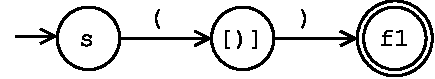
\includegraphics{fig/finiteAutomat2.pdf}
  \end{figure}

  Tento automat bude fungovat bez problému pro řetězec '()',
  my ale chceme zpracovávat i zanořené závorky a na to tento automat zatím nestačí.
  Pokud tedy chceme univerzálnější automat, stačí přidat další stav:

  \begin{figure}[H]
    \centering
    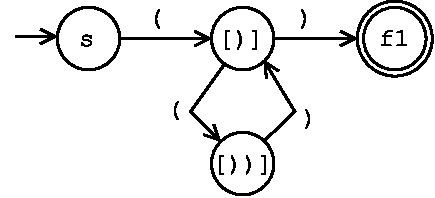
\includegraphics{fig/finiteAutomat2_1.pdf}
  \end{figure}

  Zde již zvládneme i závorky s jedním zanořením. Problémem ovšem je, že
  pro každé nové zanoření musíme přidat nový stav.
  Kdybychom tedy chtěli zpracovávat jakýkoliv počet zanoření (tedy potenciálně $\infty$),
  musel by automat obsahovat nekonečné množství stavů.
  Vidíme, že problémem Konečného automatu je, že může obsahovat pouze konečný
  počet stavů (a každý musíme ručně definovat).
  Zde tedy vidíme příklad jazyka, který nejde zpracovávat Konečným automatem
  a z toho vyplívá, že není ani Regulárním jazykem.
  Řekněme si rovnou, že bezkontextové jazyky tento problém řeší a k tomuto
  příkladu se ještě vrátíme.

\end{exmp}

\section{Bezkontextové jazyky}

Bezkontextový jazyk je obvykle definován Bezkontextovou gramatikou.
Jak jsme již uvedli v \term{Chomského hierarchii} (str. \pageref{chomsky:hierarchy}),
tyto gramatiky obsahují pravidla ve tvaru $A \rightarrow \gamma$, kde $A$ je neterminál a
$\gamma$ řetězec terminálů a neterminálů.

\subsection{Bezkontextové gramatiky}
\label{subsec:contextFreeGrammars}
Pokračujme nyní v příkladu \ref{exmp:brackets} a ukažme si, jak ho lze
vyjádřit pomocí bezkontextové gramatiky.\\

Chceme tedy vyjádřit výraz tvořený závorkami, pomocí gramatických pravidel.
Označme dvojici závorek jako výraz = neterminál $E$. Gramatické pravidlo tedy bude
vypadat takto:
\[E \rightarrow ()\]
Nyní bychom ale chtěli vyjádřit, že uvnitř závorek může být další výraz, to
lze udělat tímto rekurzivním způsobem:
\[E \rightarrow (E)\]
Zkusme nyní rozgenerovávat výraz E, tak jak to bylo naznačeno na Obr. \ref{img:rewriteRule},
tedy pomocí přepisování neterminálů:
\begin{lstlisting}
  1.        E
  2.       (E)
  3.      ((E))
  4.     (((E)))
  5.       ...
\end{lstlisting}
Vidíme, že zanořování, které nám dělalo problémy u regulárních jazyků, zde vyjádříme bez problému,
ještě by to však chtělo několik vylepšení.
Můžeme si všimnout, že rozgenerovávání by se vlastně mělo provádět do nekonečna,
protože neterminálu E se nyní nelze zbavit. To lze vyřešit přidáním tzv.
$\varepsilon$-pravidla:
\[E \rightarrow \varepsilon\]
To nám říká, že neterminál E je možno kdykoliv vymazat. Dále bychom ještě chtěli,
aby se za závorkou mohla vyskytovat další závorka, např. '(()())'.
Stačí přidat do výrazu další rekurzi:
\[E \rightarrow (E)E\]
Všimněme si ještě, že začínáme od symbolu $E$, který lze vymazat pomocí
$\varepsilon$-pravidla, přijímáme tedy i prázdný řetězec. Pokud bychom chtěli
vyjádřit, že celý výraz musí být alespoň v jedněch závrokách lze to udělat
přidáním speciálního počátečního pravidla:
\[S \rightarrow (E)\]
Nyní tedy budeme začínat od symbolu S. Označme si tuto gramatiku jako
$G$ a vyjádřeme ji formálně:

\begin{lstlisting}
  G = (
    {S, E},           (* // množina neterminálů *)
    {(, )},           (* // množina terminálů *)
    {                 (* // množina pravidel *)
      S $\rightarrow$ (E),
      E $\rightarrow$ (E)E,
      E $\rightarrow$ $\varepsilon$
    },
    S                 (* // počáteční symbol *)
  )
\end{lstlisting}

Je zřejmé, že bezkontextovými jazyky jsme schopni popsat mnohem
složitější jazyky, než regulárními jazyky. Daní za větší \term{vyjadřovací sílu}
je ale znatelně složitější zpracování těchto jazyků.

\subsection{Derivační strom}
\label{subsec:derivationTree}
Při aplikaci gramatiky na řetězec jde vlastně o ověření,
jestli lze z počátečního symbolu,
postupnou derivací (aplikací pravidel gramatiky) získat daný řetězec.
Mějme například gramatiku:

\begin{lstlisting}
  G = (
    {E},
    {*, +, a},
    {
      E $\rightarrow$ E*E,
      E $\rightarrow$ E+E,
      E $\rightarrow$ a
    },
    E
  )
\end{lstlisting}
\noindent
Pravidla této gramatiky lze vyjádřit pomocí elementárního stromu,
kde levá strana je kořen a pravá strana představuje jeho potomky.
Např. první pravidlo z gramatiky $G$ lze znázornit stromem takto:
\begin{figure}[H]
  \centering
  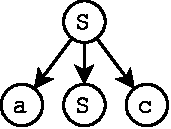
\includegraphics{fig/RuleTree1.pdf}
\end{figure}

\noindent
Pro menší velikost grafu budeme ale pravidla zjednodušeně znázorňovat takto:

\begin{figure}[H]
  \centering
  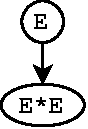
\includegraphics{fig/RuleTree2.pdf}
\end{figure}

\noindent
Pro příklad postupné derivace mějme řetězec $s$:

\begin{lstlisting}
  a * a + a
\end{lstlisting}

\noindent
Nyní zkusíme postupně aplikovat pravidla na počáteční symbol,
tak abychom získali řetězec $s$
(v komentáři jsou uvedena pravidla, která byla použita):

\begin{lstlisting}
   E
  E*E                   // E $\rightarrow$ E*E(*\footnote{Zde bychom mohli použít
    i pravidlo $E \rightarrow E + E$ a dostali bychom odlišný strom (viz. Sekce \ref{subec:nondeterminsm})}*)
  a*E                   // E $\rightarrow$ a
  a*E+E                 // E $\rightarrow$ E+E
  a*a+E                 // E $\rightarrow$ a
  a*a+a                 // E $\rightarrow$ a
\end{lstlisting}

\noindent
Touto posloupností derivací jsme byli schopni dosáhnout kontrolovaného řetězce $s$,
daný řetězec tedy patří do gramatiky. Výše zobrazené derivace lze zobrazit
i jinak a to pomocí tzv. \term{Derivačního stromu}:

\begin{figure}[H]
  \centering
  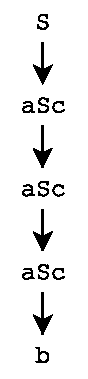
\includegraphics{fig/Derivations1.pdf}
\end{figure}

\noindent
Pro větší názornost ukažme ještě stejný strom s přiřazenými symboly k původnímu
řetězci a vyznačenými jednotlivými úrovněmi.

\begin{figure}[H]
  \centering
  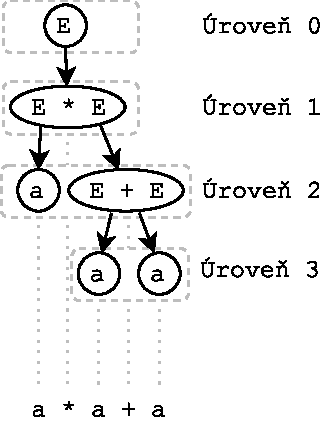
\includegraphics{fig/Derivations2.pdf}
\end{figure}

\begin{defn}
  (Derivační strom). \cite[str. 92]{MedunaIFJ}\\
  Nechť $G = (\Sigma, R)$ je Bezkontextová gramatika.\\
  \begin{enumerate}
    \item Pro $l$: $A \rightarrow x \in R, A\langle x\rangle$ je strom pravidla, které reprezentuje $l$.
    \item Derivační strom reprezentující derivace v $G$ je definován rekurzivně:
    \begin{enumerate}
      \item Strom s jedním uzlem $X$ je derivační strom odpovídající $X \Rightarrow^0 X$ v $G$, kde $X \in \Sigma$.
      \item Nechť $d$ je derivační strom reprezentující
            $A \Rightarrow^0 uBv$ [$\rho$] s hranicí($d$) $ = uBv$, a nechť $l: B \rightarrow z \in R$.
            Derivační strom, který reprezentuje
            \begin{align}
                A & \Rightarrow^* uBv [\rho] \nonumber\\
                  & \Rightarrow \hphantom{*} uzv [l] \nonumber
            \end{align}
            je získán nahrazením ($|u|+1$)-tého listu v $d$, $B$, stromem pravidla odpovídajícho $l$, $B\langle z\rangle$
    \end{enumerate}
    \item Derivační strom v $G$ je jakékoliv $t$, pro které existuje derivace odpovídající $t$ (viz 2.).
  \end{enumerate}
\end{defn}

\subsection{Nedeterminismus}
\label{subec:nondeterminsm}

U příkladu z minulé sekce (\ref{subsec:derivationTree}) si můžeme všimnout,
že při konstrukci derivačního stromu máme pro jeden řetězec možnost sestrojit
2 stromy:

\begin{figure}[H]
  \centering
  \includegraphics{fig/TwoDerivationTrees.pdf}
\end{figure}

Vidíme, že generovaný řetězec je stejný, ale stromy jsou odlišné.
Takováto gramatika je označována jako nedeterministická a způsobuje problémy při
zpracování, protože v rozhodné chvíli nevíme, které pravidlo použít.\\

Protože determinismus je při implementaci zásadní, rozdělujeme Bezkontextové gramatiky
na deterministické a nedeterministické (podobně i zásobníkové automaty).\\


\subsection{Zásobníkové automaty}

Zásobníkový automat rozšiřuje \term{Konečný automat} o zásobník, kam lze
ukládat symboly (terminály i neterminály).\\

Pro rozhodnutí, jaké pravidlo použít,
využívá vedle vstupního symbolu a stavu i symbol na vrcholu zásobníku. V rámci vykonání
přechodu lze zároveň manipulovat se zásobníkem.\\

Vraťme se opět k příkladu \ref{exmp:brackets} a všiměme si stavů
vyjadřujících zanoření. Značili jsme je jako počet uzavíracích závorek,
které jsou ještě potřeba, aby byl výraz platný. Pokud jsme narazili na
otevírací závorku, přešli jsme do stavu "o jedna více závorek", v případě uzavírací
do "o jedna méně závorek". Přechody mezi stavy jsou znázorněny na
následujícím jednoduchém řetězci:

\begin{figure}[H]
  \centering
  \includegraphics{fig/bracketsAutomat.pdf}
\end{figure}

Přidávání a odebírání závorek nám může připomínat zásobník.
Zásobníkový automat dokáže tyto stavy vyjádřit zásobníkem a potom
není nutné všechny tyto stavy definovat.\\

\begin{defn}
  (Zásobníkový automat) \cite[str. 18]{Koutny}\\
  Zásobníkový automat je sedmice $M = (Q, \Sigma, \Gamma, R, q_0, Z_0, F)$, kde:
  \begin{itemize}
    \item $Q$ je konečná množina stavů
    \item $\Sigma$ je vstupní abeceda
    \item $\Gamma$ je konečná abeceda zásobníku
    \item $R \subseteq (\Gamma \times Q \times (\Sigma \cup \{\varepsilon\} ))
    \times (\Gamma^* \cup Q)$ je konečná množina binárních relací (pravidel)
    \item $q_0 \in Q$ je počáteční stav
    \item $Z_0 \in \Gamma$ popisuje počáteční symboly na zásobníku
    \item $F \subseteq Q$ je množina konečných stavů
  \end{itemize}
\end{defn}

\noindent
Pravidla $R$ zásobníkového automatu je ve tvaru $(q_1, a, z_1) \rightarrow (q_2, \gamma)$, kde:

\begin{itemize}
  \item $q_1$ je výchozí stav
  \item $a$ je symbol na vstupu
  \item $z_1$ je symbol na vrcholu zásobníku
  \item $q_2$ je výstupní stav
  \item $\gamma$ je řetězec, který se má vložit na zásobník
\end{itemize}

Zásobníkovým automatem lze zpracovávat Deterministické bezkontextové jazyky.
V případě nedeterministických musíme nějak blíže specifikovat, který z možných
stromů chceme.\\

\section{Zpracování bezkontextových jazyků}

Při zpracování bezkontextového jazyka je hlavní problematikou
sestavování konfigurace zasobníkového automatu pro danou gramatiku.
Musíme totiž gramatická (přepisovací) pravidla zanést do konfigurace
automatu tak, aby bylo vždy jasné, které použít.\\

Při návrhu syntaktického analyzátoru se vždy objeví otázka, zdali je lepší
při konstrukci derivačního stromu postupovat od kořene (shora dolů) nebo od
zkoumaného řetězce (zdola nahoru). Odpověď na tuto otázku není jednoznačná,
což je vidět i na široce používaných analyzátorech programovacích jazyků,
kdy se tato technika liší projekt od projektu.\\

V případě tohoto projektu je tomu nejinak, a proto v této části budeme rozebírat
obě alternativy, aby byly zřejmé jejich výhody i nevýhody.

\subsection{Syntaktická analýza shora dolů}

Nejpoužívanějším zástupcem této skupiny je LL syntaktická analýza, která analyzuje
vstup zleva doprava a konstruuje nejlevější derivaci. Tato syntaktická analýza
umožňuje zpracovávat pouze LL gramatiky,
které jsou podmnožinou deterministických bezkontextových gramatik.
Pro mnoho použití není však toto omezení zásadní.\\

Které pravidlo použít slouží tzv. LL tabulka, která nám na základě
vstupního symbolu a symbolu na zásobníku určí pravidlo, které se má použít.
Následující algoritmy slouží k její konstrukci.\\

\noindent
Množina $Empty(X)$ nám říká, jestli lze symbol $X$ odstranit:\\
\begin{algorithm}[H]
  \caption{$Empty(X)$}
  \KwIn{Gramatika $G = (N, \Sigma, P, S)$}
  \KwOut{$Empty(X)$ pro každý symbol $X \in N \cup \Sigma$ }

  \BlankLine
  \Begin{
    $Empty(a) := \emptyset$ pro každé $a \in \Sigma$\;
    \ForAll{$A \in N$}{
      \uIf{$A \rightarrow \varepsilon \in P$}{
        $Empty(A)$ := $\{\varepsilon\}$\;
      }
      \Else{
        $Empty(A)$ := $\emptyset$\;
      }
    }

    \Repeat{žádná z množin Empty nezměněna} {
      \If{$A \rightarrow X_1 X_2 ... X_n \in P$ \And   $Empty(X_i) = {\varepsilon}$
              pro všechna $i = 1, ... ,n$}{
        $Empty(A)$ := $\{\varepsilon\}$\;
      }
    }
  }
\end{algorithm}
\vspace{0.5cm}

\noindent
Množina $First(X)$ nám říká, které terminální symboly se mohou nacházet
na začátku symbolu $X$:\\
\begin{algorithm}[H]
  \caption{$First(X)$}
  \KwIn{Gramatika $G = (N, \Sigma, P, S)$}
  \KwOut{$First(X)$ pro každý symbol $X \in N \cup \Sigma$ }

  \BlankLine
  \Begin{
    $first(a) := \{a\}$\ pro každé $a \in \Sigma$\;
    $first(A) := \emptyset$ pro každé $A \in N$\;

    \Repeat{žádná z množin $First$ nezměněna} {
      \If{$A \rightarrow X_1 X_2 ... X_{k-1}X_k ... X_n \in P$}{
        $First(A)$ := $First(A) \cup First(X_1)$\;
        \If{$Empty(X_i) = \{\varepsilon\}$
            pro $i = 1, ..., k-1$ kde $k \leq n$}{
          $First(A)$ := $First(A) \cup First(X_k)$\;
        }
      }
    }
  }
\end{algorithm}
\vspace{0.5cm}

\noindent
Množina $Empty(X_1X_2 ... X_n)$ nám říká, jestli lze řetězec
$X_1X_2 ... X_n$ odstranit:\\
\begin{algorithm}[H]
  \caption{$Empty(X_1X_2 ... X_n)$}
  \KwIn{Gramatika $G = (N, \Sigma, P, S)$; $Empty(X)$
        pro každé $X \in N \cup T$; $x = X_1X_2 ... X_n$,
        kde $x \in (N \cup T)^+$}
  \KwOut{$Empty(X_1X_2 ... X_n)$}

  \BlankLine
  \Begin{
    \uIf{$Empty(X_i) = \{\varepsilon\}$ pro každé $i = 1, ..., n$}{
      $Empty(X_1X_2 ... X_n)$ := $\{\varepsilon\}$\;
    }
    \Else{
      $Empty(X_1X_2 ... X_n)$ := $\emptyset$\;
    }
  }
\end{algorithm}
\vspace{0.5cm}

\noindent
Množina $First(X_1X_2 ... X_n)$ nám říká, které terminální symboly
se mohou nacházet na začátku řetězce $X_1X_2 ... X_n$:\\
\begin{algorithm}[H]
  \caption{$First(X_1X_2 ... X_n)$}
  \KwIn{Gramatika $G = (N, \Sigma, P, S)$; $First(X)$ a $Empty(X)$
        pro každé $X \in N \cup T$; $x = X_1X_2 ... X_n$,
        kde $x \in (N \cup T)^+$}
  \KwOut{$First(X_1X_2 ... X_n)$}

  \BlankLine
  \Begin{
    $First(X_1X_2 ... X_n)$ := $First(X_1)$\;

    \Repeat{množina $First(X_1X_2 ... X_{k-1}X_k ... X_n)$ nezměněna} {
      \If{$Empty(X_i) = \{\varepsilon\}$
          pro $i = 1, ..., k-1$ kde $k \leq n$}{
        $First(X_1X_2 ... X_n)$ := $First(X_1X_2 ... X_n) \cup First(X_k)$\;
      }
    }
  }
\end{algorithm}
\vspace{0.5cm}

\noindent
Množina $Follow(X)$ říká, které terminální symboly se mohou nacházet
za symbolem $X$:\\
\begin{algorithm}[H]
  \caption{$Follow(X)$}
  \label{alg:follow}
  \KwIn{Gramatika $G = (N, \Sigma, P, S)$}
  \KwOut{$Follow(A)$ pro každý symbol $A \in N$}

  \BlankLine
  \Begin{
    $Follow(S) := \{\$\}$\;

    \Repeat{žádná z množin $Follow$ nezměněna} {
      \If{$A \rightarrow xBy \in P$}{
        \If{$y \neq \varepsilon$}{
          $Follow(B)$ := $Follow(B) \cup First(y)$\;
        }
        \If{$Empty(y) = \{\varepsilon\}$
            pro $i = 1, ..., k-1$ kde $k \leq n$}{
          $Follow(B)$ := $Follow(B) \cup Follow(A)$\;
        }
      }
    }
  }
\end{algorithm}
\vspace{0.5cm}

\noindent
Množina $Predict(A \rightarrow x)$ říká, které terminální symboly mohou být
na vstupu pro pravidlo $A \rightarrow x$:
\begin{defn}
  (Množina $Predict(A \rightarrow x)$)\\
  Nechť $G = (N, \Sigma, P, S)$ je Bezkontextová gramatika.
  Pro každé $A \rightarrow x \in P$ definujeme množinu
  $Predict(A \rightarrow x \in P)$ takto:
  \begin{description}
    \item[Pokud $Empty(x) = \{\varepsilon\}$ potom:]\hfill \\
    $Predict(A \rightarrow x \in P) = First(x) \cup Follow(A)$
    \item[Jinak:]\hfill \\
    $Predict(A \rightarrow x \in P) = First(x)$
  \end{description}
\end{defn}
\vspace{0.5cm}

\noindent
Zbývá už jen naplnit LL tabulku pro funkci $\alpha(A, a)$, která nám pro neterminál
a terminál vrátí pravidlo, které použít:\\
\begin{algorithm}[H]
  \caption{$\alpha(A, a)$}
  \KwIn{Gramatika $G = (N, \Sigma, P, S)$; $Predict(A \rightarrow x)$, pro každé pravidlo z $P$}
  \KwOut{$\alpha(A, a)$, pro všechny platné kombinace $(A, a)$}

  \BlankLine
  \Begin{
    \ForAll{$A \rightarrow a \in P$} {
      \ForAll{$b \in Predict(A \rightarrow a)$}{
        \uIf{$\alpha(A, b)$ není definováno}{
          $\alpha(A, b) = A \rightarrow a$
        }
        \Else{
          chyba - nejde o LL gramatiku
        }
      }
    }
  }
\end{algorithm}
\vspace{0.5cm}

Chybový stav v posledním algoritmu nám vlastně indikuje nedeterminismus
v LL tabulce - tedy že pro nějakou kombinaci $A, a$ by v LL tabulce bylo
více záznamů, takže bychom nevěděli, které pravidlo použít.\\

\begin{exmp}
Vraťme se nyní ke gramatice $G$
(z kapitoly \ref{subsec:contextFreeGrammars}):

\begin{lstlisting}
  G = (
    {S, E},           (* // množina neterminálů *)
    {(, )},           (* // množina terminálů *)
    {                 (* // množina pravidel *)
      S $\rightarrow$ (E),         (* // pravidlo 1 *)
      E $\rightarrow$ (E)E,        (* // pravidlo 2 *)
      E $\rightarrow$ $\varepsilon$             (* // pravidlo 3 *)
    },
    S                 (* // počáteční symbol *)
  )
\end{lstlisting}
\noindent
LL tabulku bychom podle výše uvedených algoritmů sestavili takto:
\begin{table}[H]
  \centering
  \begin{tabular}{| c || c | c | c |}
    \hline
      & ( & ) & \$ \\
    \hhline{|=||=|=|=|}
    S & 1 &   &    \\
    \hline
    E & 2 & 3 &    \\
    \hline
  \end{tabular}
  \caption{LL tabulka gramatiky G s čísly pravidel}
\end{table}


Nyní zkusme zpracovat řetězec \texttt{'(())'} gramatikou $G$
s pomocí LL tabulky.
Vlevo je znázorněný zásobník (s vrcholem)
a šipky ukazují na aktuální vstupní symbol.
Speciální znak '\$' nám značí konec vstupu.

\begin{figure}[H]
  \centering
  \subfloat[Zpracování řetězce]{
    \includegraphics[scale=0.6]{fig/bracketsCFAutomat.pdf}
  }
  \subfloat[Derivační strom]{
    \hspace{1cm}
    \includegraphics{fig/bracktesDerivationTree.pdf}
    \hspace{1cm}
  }
\end{figure}

Při zpracování jsme postupovali tak jako zásobníkový automat.
Před zahájením algoritmu vložíme na zásobník symbol '\$'
a počáteční symbol 'S'. Vysvětleme podrobně některé kroky (číslování odpovídá obrázku):

\begin{itemize}
  \item[1.] Na zásobníku je neterminál 'S' - na základě vstupu '(' vybereme
  z LL tabulky pravidlo 1 a nahradíme S za pravou stranu pravidla
  \item[2.] Na zásobníku je terminál '(' a shoduje se se vstupním symbolem - můžeme jej odstranit
  \item[3.] Na zásobníku je neterminál 'E' a na vstupu opět '(', použijeme pravidlo 2
  \item[4.] Na zásobníku je terminál '(' a shoduje se se vstupem - odstraníme
  \item[5.] Na zásobníku je neterminál 'E' a na vstupu ')' - použijeme pravidlo 3
  \item[] ...
  \item[9.] Na zásobníku je terminál '\$' a shoduje se se vstupem - při tomto znaku skončíme
\end{itemize}
\end{exmp}

\noindent
Při zpracování mohou nastat následující chyby:

\begin{itemize}
  \item Znak na vstupu není v abecedě
  \item V LL tabulce není pravidlo pro danou kombinaci neterminálu a terminálu
  \item Terminály na vstupu a vrcholu zásobníku se neschodují
\end{itemize}

\noindent
Všechny tyto případy znamenají, že řetězec nepatří do gramatiky $G$

\subsection{Syntaktická analýza zdola nahoru}

Syntaktická analýza zdola nahoru sestavuje derivační strom odspodu,
tedy začíná neterminály a postupně se propracuje až k počátečnímu symbolu
gramatiky.


\subsubsection*{LR syntaktická analýza}
Pro účely této práce se budeme zabývat LR syntaktickou analýzou, jelikož
parsery tohoto typu mají sílu ekvivalentní s \term{Deterministickým zásobníkovým
automatem}\cite[str. 155]{MedunaIFJ}, tedy představují nejsilnější nástroj
v oblasti \term{Deterministických bezkontextových jazyků}.
LR syntaktická analýza generuje obrácený pravý rozbor.\\

Pro zpracování se opět používá \term{Zásobníkový automat}, který je
rozšířen o možnost pracovat na vrcholu zásobníku s řetězecem (ne jen s jedním symbolem).
Toto rozšíření je nutné pro aplikování pravidel - tedy nahrazení řetězce na pravé straně za
symbol na levé straně pravidla (postupujeme opačně než u LL).\\

Při analýze řetězce dáváme postupně příchozí symboly na zásobník (operace \term{shift})
a v určité chvíli použijeme pravidlo a nahradíme symboly na vrcholu zásobníku za
jeho levou stranu (operace \term{reduce}). Kterou operaci v dané chvíli provést
nám určuje tzv. LR tabulka, jejíž konstrukcí se budeme dále zabývat.\\

\subsubsection*{LR tabulka}

LR tabulka je poněkud složitější, než LL tabulka. Obsahuje 2 části:

\begin{itemize}
  \item Akční část je definována jako $\alpha(q, a)$ kde $q$ je stav a $a$ je terminál.\\
  Určuje jakou operaci provést a k tomu informaci
  do jakého stavu přejít (u op. shift) nebo jaké pravidlo použít (op. reduce), a také speciální
  ukončovací symbol
  \item Přechodová část je definována jako $\beta(q, A)$ kde $q$ je stav a $A$ je neterminál.\\
  Určuje do jakého stavu přejít po aplikaci pravidla.
\end{itemize}

Stav zde vyjadřuje možnosti, které vyplívají ze znaků naposledy přečtených.
Pro každý stav existuje množina pravidel, jejichž pravá strana prozatím vyhovuje přečteným symbolům.
Při znázorňování množin pravidel budeme používat znak '•' znázorňující aktuální pozici v pravidle.\\

\noindent
Algoritmus $Closure(I)$ je definován pro pravidlo s určenou pozicí a generuje z něj stavovou skupinu:\\
\begin{algorithm}[H]
  \caption{$Closure(I)$}
  \KwIn{Gramatika $G = (N, \Sigma, P, S)$; Položka $I$}
  \KwOut{$Closure(I)$}

  \BlankLine
  \Begin{
    $Closure(I)$ := $\{I\}$\;
    \Repeat{množina $Closure(I)$ nezměněna}{
      \If{$A \rightarrow y$•$Bz \in Closure(I)$ \And $B \rightarrow x \in P$} {
        $Closure(I)$ := $Closure(I) \cup B \rightarrow $ •$x$\;
      }
    }
  }
\end{algorithm}
\vspace{0.5cm}

\noindent
Následující algoritmus vytvoří množinu $\Theta_G$ všech stavových množin pro gramatiku $G$ rozšířenou o
pravidlo $S' \rightarrow S$, kde $S$ je počáteční symbol:\\
\begin{algorithm}[H]
  \caption{$\Theta_G$}
  \label{alg:groups}
  \KwIn{Rozšířená gramatika $G = (N, \Sigma, P, S')$}
  \KwOut{$\Theta_G$}

  \BlankLine
  \Begin{
    $\Theta_G$ := $\{Closure(S' \rightarrow $ •$S)\}$\;
    \ForAll{$I \in \Theta_G$ \And $U \in N \cup \Sigma$}{
      \If{$\Theta_U(I) \neq \emptyset$} {
        přidej $\Theta_U(I)$ do $\Theta_G$;
      }
    }
  }
\end{algorithm}
\vspace{0.5cm}

\noindent
Nyní sestrojíme LR tabulku, pomocí SLR algoritmu. Budeme zde potřebovat také
algoritmus \ref{alg:follow} ($Follow$). Operaci shift znázorňujeme jako $s$,
reduce jako $r$. Ukončovací symbol označme jako a (accept).\\
\begin{algorithm}[H]
  \caption{$SLR$}
  \KwIn{Rozšířená gramatika $G = (N, \Sigma, P, S')$;
    $\Theta_G;$ $Follow(A)$ pro všechna $A \in N$}
  \KwOut{LR tabulka pro $G$ ($\alpha$ = akční č., $\beta$ = přechodová č.)}

  \BlankLine
  \Begin{
    \ForAll{$x \in \Theta_G$}{
      \ForAll{$I \in x$}{
        \Switch{$I$}{
          \Case{$I = A \rightarrow y$•$Xz$, kde $X \in N$:}{
            $\beta[x, X] := \Theta_X(x)$ \tcp*{$\beta$ část}
          }
          \Case{$I = A \rightarrow y$•$Xz$, kde $X \in \Sigma$:}{
            $\alpha[x, X] := s\Theta_X(x)$ \tcp*{operace shift}
          }
          \Case{$I = S' \rightarrow S$•:}{
            $\alpha[x, \$]$ := a  \tcp*{úspěšný konec}
          }
          \Case{$A \rightarrow y$• $(A \neq S')$:}{
            \ForAll{$a \in Follow(A)$}{
              $\alpha[x, a]$ := $rp$,
              kde $p$ je číslo pravidla $A \rightarrow y$ \tcp*{reduce}
            }
          }
        }
      }
    }
  }
\end{algorithm}
\vspace{0.5cm}

\noindent
Syntaktická analýza využívající LR tabulku vypadá takto:\\
\begin{algorithm}[H]
  \caption{LR syntaktická analýza}
  \label{alg:lr}
  \KwIn{LR tabulka pro $G = (N, \Sigma, P, S)$ a řetězec $x \in T^*$}
  \KwOut{Pravý rozbor $x$, pokud $x \in L(G)$, jinak chyba}

  \BlankLine
  \Begin{
    Vlož $\langle\$,q_0\rangle$ na zásobník\;
    $stav$ := $q_0$\;
    \Repeat{úspěch \Or chyba}{
      $a$ = aktuální znak na vstupu\;
      \Switch{$\alpha[stav, a]$}{
        \uCase{$sq$:}{
          push($\langle a, q\rangle$)\;
          přečti další znak $a$ ze vstupu\;
          stav := q\;
        }
        \uCase{$rp$}{
          \uIf{$p$: $A \rightarrow X_1X_2 ... X_n \in P$ \And
            $\langle?,q\rangle\langle X_1, ?\rangle\langle X_2, ?\rangle ... \langle X_n, ?\rangle$
              je na vrcholu zásobníku}{
            $stav$ := $\beta[q,A]$\;
            zaměň na zásobníku $\langle X_1, ?\rangle\langle X_2, ?\rangle ... \langle X_n, ?\rangle$
              za $\langle A, stav\rangle$\;
            zapiš $p$ na výstup\;
          }
          \Else{
            chyba
          }
        }
        \uCase{a}{
          úspěch
        }
        \Case{nedefinováno}{
          chyba
        }
      }
    }
  }
\end{algorithm}
\vspace{0.5cm}

\begin{exmp} Vezměme gramatiku $G$ z kapitoly \ref{subsec:derivationTree}:


\begin{lstlisting}
  G = (
    {E},
    {*, +, a},
    {
      S' $\rightarrow$ E,               // pravidlo 0 (*(přidané)*)
      E $\rightarrow$ E*E,              // pravidlo 1
      E $\rightarrow$ E+E,              // pravidlo 2
      E $\rightarrow$ a                 // pravidlo 3
    },
    E
  )
\end{lstlisting}

\noindent
Stavové skupiny $\Theta_G$ z algoritmu \ref{alg:groups} pro tuto gramatiku vypadají takto:
\begin{lstlisting}
  0: S' -> (*•*)E, E -> (*•*)E*E, E -> (*•*)E+E, E -> (*•*)a
  1: S' -> E(*•*), E -> E(*•*)*E, E -> E(*•*)+E
  2: E -> a(*•*)
  3: E -> E*(*•*)E, E -> (*•*)E*E, E -> (*•*)E+E, E -> (*•*)a
  4: E -> E+(*•*)E, E -> (*•*)E*E, E -> (*•*)E+E, E -> (*•*)a
  5: E -> E*E(*•*), E -> E(*•*)*E, E -> E(*•*)+E
  6: E -> E+E(*•*), E -> E(*•*)*E, E -> E(*•*)+E
\end{lstlisting}

\noindent
Zde je LR tabulka:

\begin{table}[H]
  \centering
  \begin{tabular}{| c || c | c | c | c || c | c |}
    \hline
      & * & + & a & \$& S'& E \\
    \hhline{|=||=|=|=|=||=|=|}
    0 &   &   & s1 &   &   & 2 \\
    \hline
    1 & r3 & r3 &   & r3 &   &   \\
    \hline
    2 & s3 & s4 &   & a &   &   \\
    \hline
    3 &   &   & s1 &   &   & 5 \\
    \hline
    4 &   &   & s1 &   &   & 6 \\
    \hline
    5 & s3 r1 &  s4 r1 & & r1 &   & \\
    \hline
    6 & s3 r2 &  s4 r2 & & r2 &   & \\
    \hline
  \end{tabular}
\end{table}

Všimněme si, že v některých polích tabulky máme 2 položky. Tyto případy
se nazývají \term{shift-reduce} konflikty a jsou projevem toho, že je tato
gramatika nedeterministická (viz. sekce \ref{subec:nondeterminsm}).
Výhodou LR gramatiky je to, že ji lze lehce rozšířit o priority operátorů
a poté za běhu rozhodnout, které pravidlo použít.
Priority pro tuto gramatiku mohou vypadat následovně:

\begin{lstlisting}
  left: *
  left: +
\end{lstlisting}

V tomto případě má tedy operátor '*' vyšší prioritu a oba operátory jsou vyhodnocovány zleva.
Za běhu poté porovnáváme příchozí neterminál s posledním operátorem na zásobníku
a na základě toho rozhodneme jestli provedeme operaci \term{shift} nebo \term{reduce}.
Ukažme si zpracování řetězce '\texttt{a * a + a}':

\begin{figure}[H]
  \centering
  \subfloat[Zpracování řetězce]{
    \includegraphics[scale=0.6]{fig/exprLRParsing.pdf}
  }
  \subfloat[Derivační strom]{
    \hspace{1cm}
    \includegraphics{fig/exprDerivationTree.pdf}
    \hspace{1cm}
  }
\end{figure}

Ve výše zobrazeném diagramu postupujeme podle algoritmu \ref{alg:lr},
vysvětleme některé kroky:
\begin{itemize}
  \item[1.] Jsme ve stavu 0 a na vstupu máme 'a' - podle LR tabulky přejdeme do
  stavu 1 a provedeme operaci \term{shift} (vložíme 'a' na zásobník s aktuálním stavem).
  \item[2.] Jsme ve stavu 1 a na vstupu máme '*' - podle LR tabulky provedeme
  operaci \term{reduce} podle pravidla 3 - poslední stav za nahrazovanou částí na
  zásobníku je 0 a levá strana pravidla je 'E' - podle beta části LR tabulky
  přejdeme do stavu 2 (vložíme na zásobník i s neterminálem E).
  \item[3.] Jsme ve stavu 2 a na vstupu máme '*' - \term{shift} 3.
  \item[4.] Jsme ve stavu 3 a na vstupu máme 'a' - \term{shift} 1.
  \item[5.] Jsme ve stavu 1 a na vstupu máme '+' - \term{reduce} 3
   - poslední stav je 3 a levá strana je 'E' - přejdeme do stavu 5.
  \item[6.] Jsme ve stavu 5 a na vstupu máme '+' - narazili jsme na \term{shift-reduce} konflikt
  v LR tabulce - poslední operátor na zásobníku je '*', protože má vyšší prioritu,
  provedeme operaci \term{reduce} 1 - poslední stav je 0 a levá strana je 'E' - přejdeme do stavu 2.
  \item[] ...
  \item[11.] Jsme ve stavu 2 a na vstupu máme '\$' - V LR tabulce je \texttt{a}
  (Accept) - můžeme skončit a řetězec prohlásit za přijatý.
\end{itemize}
\end{exmp}

Je vidět, že pomocí LR syntatické analýzy jsme schopni zpracovávat deterministické
gramatiky a pokud přidáme priority, i některé nedeterministické. Všimněme si jak je
sestavován derivační strom - jdeme odspodu a vytváříme několik podstromů,
teprve v posledním kroku je spojíme do jednoho.


\chapter{Zpracování jazyků řízených stromy}
\label{ch:processingTreeLanguages}

\section{Omezení úrovní derivačního stromu}

V této části práce je vysvětleno, jak lze omezit derivační stromy a tím zvýšit
sílu dané gramatiky.
Teoretická část této kapitoly vychází převážně z práce Ing. Koutného\cite{Koutny}.\\

\begin{defn}
  (Gramatiky řízené stromy) \cite[str. 28]{Koutny}\\
  Gramatika řízená stromem je dvojice $(G, R)$, kde $G = (V, T, P, S)$
  je řízená gramatika a $R \subseteq V^*$ kontrolní jazyk.
\end{defn}

\begin{defn}
  (Jazyky řízené stromy) \cite[str. 28]{Koutny} \label{jazykyRS}\\
  Nechť $(G, R)$ je gramatika řízená stromem.
  Jazyk generovaný $(G, R)$ je značen jako $L(G, R)$ a definován jako:
  \vspace{5pt}
  \begin{adjustwidth}{0.5cm}{0.5cm}
    $L(G, R) = \{x: x \in L(G, R)$ a existuje derivační strom $t$ pro
    každé $x$ v $G$ takový, že každé slovo získané konkatenací
    všech symbolů na kterékoliv úrovni $t$ (kromě poslení) zleva doprava,
    patří do $R \}$.
  \end{adjustwidth}
\end{defn}

\noindent
V této práci se zabýváme především gramatikami bezkontextovými, protože
je lze relativně snadno zpracovávat a kontrolní jazyk bude regulární.
Jinými slovy, zabýváme se gramatikami $(G, R)$, kde G je bezkontextová gramatika
a R je regulární jazyk.

\subsection{Příklady}

Pro lepší porozumění následuje podrobný praktický příklad, jak lze
ověřovat příslušnost řetězce do dané gramatiky řízené stromem.

\begin{exmp}
  Mějme stromem řízený jazyk $L(G, R)$, kde:
  \begin{lstlisting}
  G = (
    {S, A, B, C, a, b, c},
    {a, b, c},
    {
      S $\rightarrow$ ABC,
      A $\rightarrow$ aA,
      A $\rightarrow$ a,
      B $\rightarrow$ bB,
      B $\rightarrow$ b,
      C $\rightarrow$ cC,
      C $\rightarrow$ c
    },
    S
  ),
  R = {S, ABC, aAbBcC}
  \end{lstlisting}
  \noindent
  A řetězec:

  \begin{lstlisting}
  aabbcc
  \end{lstlisting}

  \noindent
  Nejprve sestavíme derivační strom pro daný řetězec, poté projdeme všechny
  jeho úrovně (kromě poslední, viz. Definice \ref{jazykyRS}) a
  ověříme, že patří do kontrolního jazyka $R$.

  \begin{figure}[H]
    \centering
    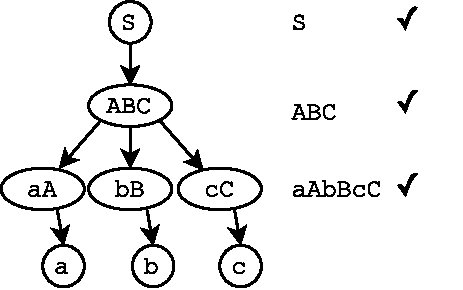
\includegraphics{fig/TreeControlledGrammar1.pdf}
  \end{figure}

  \noindent
  Z grafu je zřejmé, že v tomto případě řetězec patří do jazyka $L$.
  Zkusme však ještě jiný případ pro tento řetězec:

  \begin{lstlisting}
  aabcc
  \end{lstlisting}

  \noindent
  A jemu odpovídající derivační strom:
  \begin{figure}[H]
    \centering
    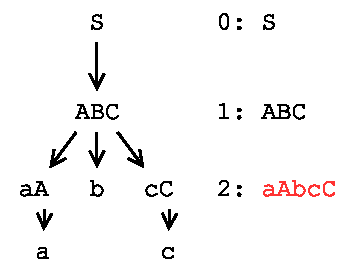
\includegraphics{fig/TreeControlledGrammar2.pdf}
  \end{figure}

  \noindent
  V tomto případě úroveň 2 derivačního stromu nepatří do kontrolního jazyka $R$,
  proto tento řetězec nepatří do jazyka $L$.
\end{exmp}

\chapter{Implementace}

%=========================================================================
